%\section{Specialized question answering}
%\label{sec:related_work_emnlp2016}

A common model for question answering (QA) is that a good answer is one that is closely related to the question, where relatedness is often determined using general-purpose lexical models such as word embeddings. 
Here we argue that a better approach is to look for answers that are related to the question in a {\em relevant way}, according to the information need of the question (that is, the question type).
In this way, a QA system might consist of many distinct solvers, each specialized to the inference needs of a particular question type, such as causal inference or reasoning over a process\footnote{\rev{Not addressed here is \textit{how} questions are to be classified, and it is very much open-ended. Not only is the \textit{number} of classes open-ended, but also the \textit{type} of the classes themselves -- for example you could base them on domain (e.g., Biology versus Geology, etc.), or, as discussed here the inference type required (e.g., causal versus definitional, etc.), or some other dimension entirely.  Even after determining a classification scheme, developing the classifier itself is certainly non-trivial, made more difficult by the fact that complex questions can potentially belong to several different classes, as described by \citet{jansen-EtAl:2016:COLING}.  However, this is beyond the scope of the current work.}}.  Here we explore one framework that could be used for these solvers, which we use to answer causal questions.  We argue that this general framework can be extended easily to handle other question types.

\section{Related Work} 
%\subsection{Specialized question answering}
We are not the first to assert the need for specialized solving methods in QA.  For example, \citet{oh2013question} incorporate a dedicated causal component into their system, and note that it improves the overall performance.  However, their model is limited by the need for explicit lexical overlap between a causal construction found in their knowledge base and the question itself.  Here, we develop a causal QA component that exploits specialized word embeddings that are task-specific (i.e., specifically learned to model the desired semantic relation, here \textit{causality}), to gain robustness to lexical variation.  
By using word embeddings, we can model the likelihood of a causal link between two texts even when the exact lexical items were never observed together in the knowledge base.

%\subsection{Embeddings for question answering}
% Embeddings in QA
There has been a vast body of work which demonstrates that word embeddings derived from distributional similarity are useful in many tasks, including question answering~\mbox{\citep[see \emph{inter alia}][]{fried2015higher,yih13}}.  However, \citet{levy2015supervised} note that there are limitations on the type of semantic knowledge which is encoded in these general-purpose similarity embeddings.  Therefore, rather than limit ourselves to the general purpose embeddings, here we build task-specific embeddings that are customized for answering causal questions.

%\subsection{Customizing embeddings}
%% Customized embeddings
Customized embeddings have been created for a variety of tasks. %including semantic role labeling~\citep{fitzgerald2015semantic,woodsenddistributed}, and binary relation extraction ~\mbox{\citep{riedel2013relation}.}
For example, with semantic role labelling, custom embeddings have been learned for semantic frames, their arguments, and the roles of the arguments~\citep[e.g.,][]{fitzgerald2015semantic,woodsenddistributed}.  \citet{riedel2013relation} used distant supervision to learn embeddings for binary relations (such as \textit{employed\_by}) and argument pairs (such as $<$\textit{Jane Smith, Harvard}$>$) in order to perform automated database completion.  
Similar to \citeauthor{riedel2013relation}, we train embeddings customized for specific relations, but we bootstrap training data using minimal supervision (i.e., a small set of patterns) rather than relying on distant supervision and large existing knowledge bases.  Additionally, while Riedel et al. represent \textit{all} relations in a general embedding space, here we train a dedicated embedding space for just the causal relations. 

For use in question answering, embeddings have been customized to have question words that are close to either their answer words~\citep{bordes2014question}, or to structured knowledge base entries~\citep{yang2014joint}.  While these methods are useful for QA, they do not distinguish between different types of questions, and as such their embeddings are not specific to a given question type.

Additionally, embeddings have been customized to distinguish functional similarity from relatedness ~\citep{levy2014dependency,kielaspecializing}.
In particular, Levy and Goldberg train their embeddings by replacing the standard linear context of the target word with context derived from the syntactic dependency graph of the sentence.  The resulting embeddings, they argue, model functional similarity rather than topical similarity.  For example, when given the word \emph{turing}, wheras a traditional embeddings model returns top associates containing topically related words such as \emph{non-deterministic} and \emph{finite-state}, the dependency-based model returns other tests (i.e., \emph{pauling, hotelling,} and \emph{hamming}).
In this work, we make use of this extension to arbitrary context in order to train our embeddings with contexts derived from binary causal relations.  We extract cause-effect text pairs such that the cause text becomes the \emph{target} text and the effect text serves as the \emph{context}. This raises the issue of multiword target and context texts, which we address in Section \ref{sec-emnlp2016:models}.

%\subsection{Evaluating embeddings} 
Recently, \citet{faruqui2016problems} discussed issues surrounding the evaluation of similarity word embeddings, including the lack of correlation between their performance on word-similarity tasks and ``downstream'' or real-world tasks like QA, text classification, etc.  As they advocate, in addition to a direct evaluation of our causal embeddings (see Section \ref{sec-emnlp2016:directeval}), we also evaluate them independently in a downstream QA task (Section \ref{sec-emnlp2016:indirecteval}).  We provide the same comparison for two alternative approaches (an alignment model and a convolutional neural network model), confirming that the direct evaluation performance can be misleading without the task-specific, downstream evaluation.

%\subsection{Extracting Causal Text}
With respect to extracting causal relations from text, Girju et al.~\citeyear{girju2002text} use modified Hearst patterns~\cite{hearst1992automatic} to extract a large number of potential cause-effect tuples, where both causes and effects must be nouns.
However, Cole et al.~\citeyear{cole2005lightweight} show that these nominal-based causal relations account for a relatively small percentage of all causal relations, and for this reason, \cite{yang2014multi} allow for more elaborate argument structures in their causal extraction by identifying verbs, and then following the syntactic subtree of the verbal arguments to construct their candidate causes and effects. 
Additionally, Do et al.~\citeyear{do2011minimally} observe that nouns as well as verbs can signal causality.  
We follow these intuitions in developing our causal patterns by using both nouns and verbs to signal potential participants in causal relations, and then allowing for the entire dominated structures to serve as the cause and/or effect arguments.

\section{Chapter overview}

The rest of the Chapter is organized as follows.  
%In Section \ref{sec-emnlp2016:approach} we outline our approach to generating and using causal embeddings for question answering.  
In Section \ref{sec-emnlp2016:causalextraction} we provide details concerning our semi-supervised methods for gathering a large number of cause-effect text pairs that we use for training our models.  In Section \ref{sec-emnlp2016:models} we describe our primary causal embedding models as well as several other variants.  In Section \ref{sec-emnlp2016:directeval} we evaulate these models directly on a causal-relation identification task.  Then, in Section \ref{sec-emnlp2016:indirecteval} we detail the experimental setup for our indirect evaluation: causal QA over a subset of Yahoo! Answers.  We show that explicitly modeling causality improves performance in both the direct and the indirect tasks. In the QA task our best model achieves 37.3\% P@1, significantly outperforming a strong baseline by 7.7\% (relative).
We also show that the results of these two evaluations are \emph{not} identical: a given model's performance on the direct evaluation does not necessarily transfer to the more complex, real-world QA task, as discussed in our conclusions in Section \ref{sec-emnlp2016:conclusion}.


%\begin{figure}[t!]
%\begin{center}
%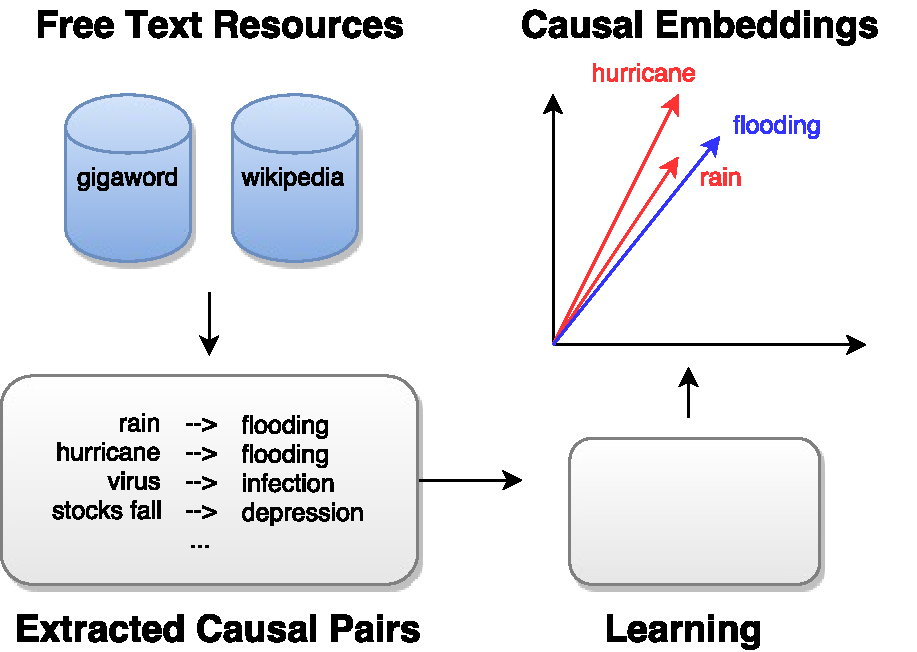
\includegraphics[width=75mm]{emnlpArchDraft.pdf}
%%\vspace{-4mm}
%\caption{{\small Our proposed pipeline for training a causal embedding space from free text resources. \todo{fill in learning with final model}}}
%\vspace{-6mm}
%\label{fig:arch}
%\end{center}
%\end{figure}
%
%\section{Approach}
%\label{sec-emnlp2016:approach}
%%\vspace{-2mm}
%
%Our focus is on reranking answers to causal questions using using task-specific distributional similarity methods.
%%on the the task of question answering, which is complicated by the variety of question types (e.g., definitional, causal),  each having different information needs that potentially require dedicated solving methods~\cite{clark2013study}.  
%%Longer term, we propose a QA approach which uses dedicated, task-specific word embeddings for each question type, aimed at maintaining the robustness of word embeddings while gaining the specificity of dedicated solving methods. 
%%Here, we address one particular information need: causality.
%%
%Our approach operates in three steps:
%
%{\flushleft (1)} We start by bootstrapping a large number of cause-effect pairs from free text using a small number of syntactic and surface patterns (Section \ref{sec-emnlp2016:causalextraction}).
%
%{\flushleft (2)} We then use these bootstrapped pairs to build several task-specific embedding (and other distributional similarity) models (Section \ref{sec-emnlp2016:models}). We evaluate these models directly on a causal-relation identification task (Section \ref{sec-emnlp2016:directeval}).  
%
%{\flushleft (3)} Finally, we incorporate these models into a reranking framework for causal QA and demonstrate that the resulting approach performs better than the reranker without these task-specific models, even if trained on the same data (Section ~\ref{sec-emnlp2016:indirecteval}).  


%We approach the task of creating and evaluating a task-specific relational vector space by considering one relation in particular -- causality.  The architecture of our system is shown in Figure \ref{fig:arch}. \todo{do I really need an architecture here?}

%rule-based framework which analyzes free text and returns cause-effect tuples.  
%These pairs are then used to learn a set of high-dimensional word embeddings which are particular to the desired relation.  
%In particular, we make use of the Levy and Goldberg extension of the skipgram algorithm to learn embeddings from these pairs by predicting the effect-text given the cause-text.
%MOVE:
%using the extension of the Skipgram algorithm~\todo{cite and link} proposed by \citep{levy2014dependency}.  
%\todo{does this belong here? intro?}
%While the learning algorithm returns two distinct vector space embeddings for each item in the vocabulary, often only the target embeddings are ever used.  In this work, however, we make use of both sets of embeddings to capture the inherent \emph{directionality} of the causal relation.

%\todo{remove the evaluation info from here?}
%Once trained, we then evaluate the quality this mapping, or vector space, in two ways.  First, we evaluate it directly by attempting to rank a set of cause-effect pairs higher than entity pairs from other relations.  Second, we evaluate the mapping indirectly, by using it in the down-stream task of question answering (QA).

